\section{Performance Evaluation}
\label{2017-batched-spmv:sec:s4-experiments}

\subsection{Experiment setup}
For the performance analysis, we use the following test benchmark consisting of 32 matrices from the
SuiteSparse matrix collection~\cite{ufmc}: 
{\sc pivtol}, {\sc tomography},
{\sc west0989}, {\sc G45}, 
{\sc GD02\_a}, {\sc Si2},
{\sc ck656} {\sc ex25}, 
{\sc jgl011} {\sc lock\_700}, 
{\sc fs\_541\_1}, {\sc mbeacxc}, 
{\sc dwt\_918}, {\sc mcfe}, 
{\sc dwt\_607}, {\sc rbsa480}, 
{\sc gr\_30\_30}, {\sc bcsstk34}, 
{\sc cage8}, {\sc ex27}, 
{\sc can\_838}, {\sc bcsstm34}, 
{\sc USAir97}, {\sc bp\_1600}, 
{\sc rotor2}, {\sc msc00726}, 
{\sc nos3}, {\sc G2}, 
{\sc dwt\_992}, {\sc ex2}, 
{\sc tols90}, {\sc bcsstk02}. 
We focus on square matrices of order up to 1024, 
with real entries,
including a variety of problems
to cover a large spectrum.
Concretely, this subset contains matrices with size $n \in [11,1015]$, number of nonzeros
$nnz \in [76,38352]$, and $nnz/n \in [3.0,66.0]$.
The specific operation we target is $y := A\cdot x + y$,
which requires $2\cdot nnz$ floating-point arithmetic operations (flops),
and allows for much flexibility in terms of scaling $y$ before the
operation (e.g., scaling $y$ with 0 to compute $y=A\cdot x$).

The performance evaluation is split into three parts. 
In the first experiment, we quantify the performance advantages that the 
flexible batched routines provide
over the standard \spmv kernels when processing a homogeneous collection 
(batch) consisting
of an increasing number of identical matrices.

In the second part, we compare the batched kernels against each other, using 
homogeneous batches consisting either of the problems from the test benchmark, 
or custom-engineered matrices where we control the density and
nonzero distribution.
Although it is possible to write a much more efficient kernel for this 
problem setting (which, in particular, reuses the information about the problem 
size and the nonzero locations),
we argue that this experiment is useful to extract information about which 
format and kernel
to choose for batches containing similar problems.

In the third part of the experimental analysis, we consider batches comprising 
problems
with different characteristics. First, we look into settings where all matrices 
in the batch are of
similar size but differ in the sparsity pattern. For this purpose, we select 12 
matrices from
the test benchmark of order
800--1,024, and create the batch by appending these problems in random order.
Second, we consider batches containing any of the matrices in the test 
benchmark.

All experiments were conducted on the compute nodes of the 
PizDaint supercomputer at the Swiss National Computing Centre (CSCS). 
Although irrelevant for the performance analysis, the host contains
an Intel E5-2690 v3 (Haswell) processor with 12 cores.
All computations were executed by the NVIDIA Tesla P100 GPU (compute capability 
6.0),
using double precision arithmetic,
for which NVIDIA lists a peak performance of 5.3 TFLOPs ($10^{12}$ 
flops/second). 
The P100 is equipped with 16 GB of main memory that
are accessed at a theoretical peak bandwidth of 732 GB/s.
Using NVIDIA's CUDA toolkit version 8.0, we designed the flexible batched 
routines to be integrated into the MAGMA-sparse software 
library~\cite{parco2017}.
MAGMA-sparse was also used as experiment ecosystem, and provided
the standard \spmv reference implementations. 


\begin{figure}[t]
	\begin{center}
		\begin{tabular}{cc}
			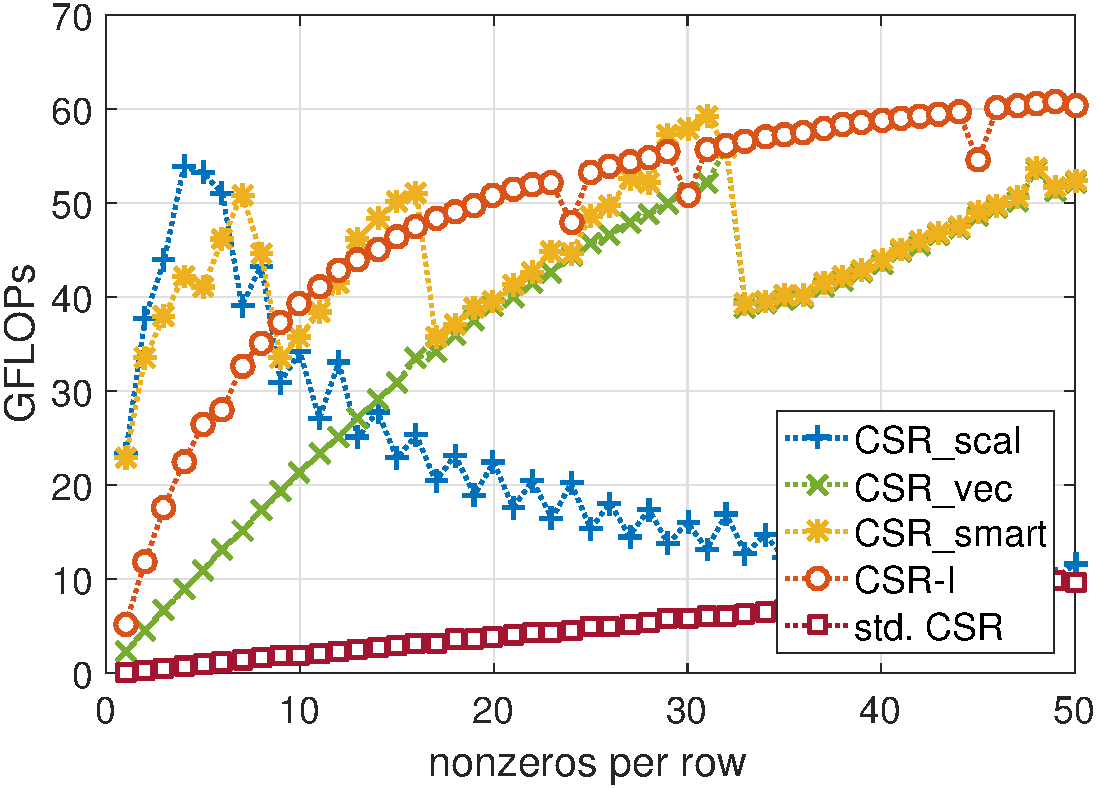
\includegraphics[width=.45\columnwidth]{plots/INCDENSITY_GFLOPS}
			&
			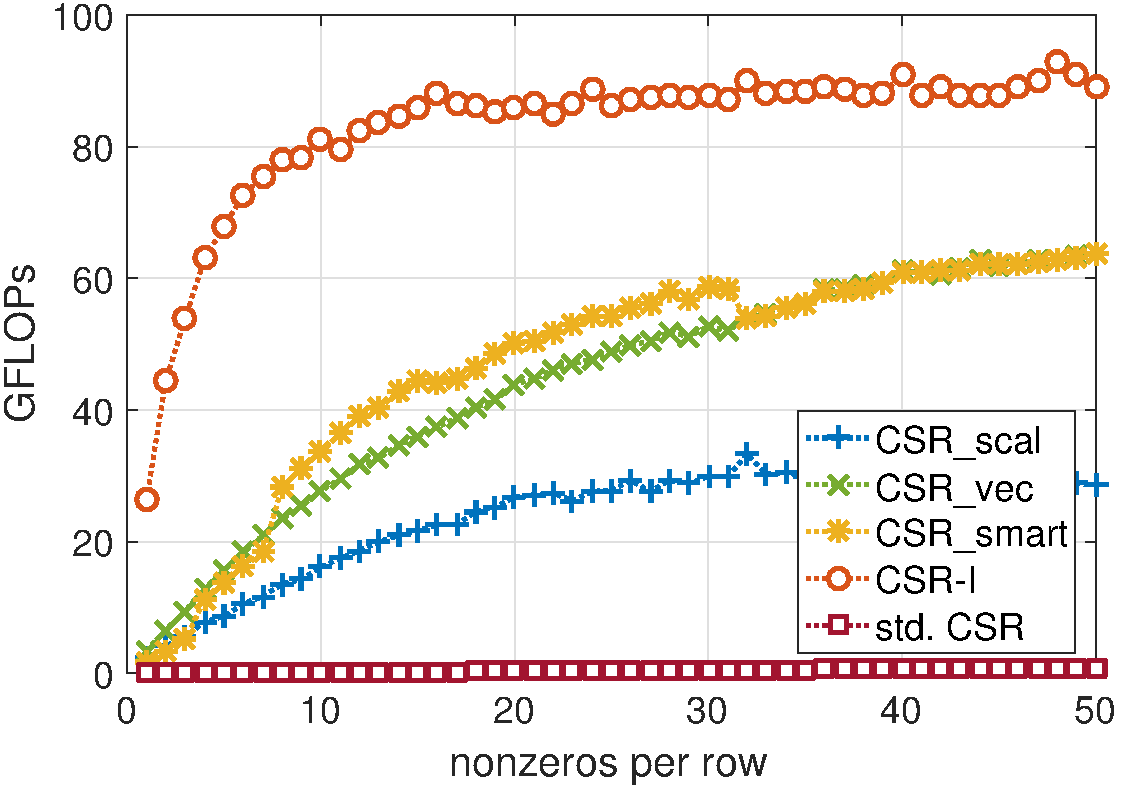
\includegraphics[width=.458\columnwidth]{plots/INC_GFLOPS}\\
		\end{tabular}
	\end{center}
	\caption
    [Performance of CSR-based \spmv routines for a homogeneous batch]
    {Performance of the standard and flexible batched CSR-based \spmv 
		routines for a homogeneous batch consisting of 1000 square matrices of 
		order 
		1024 with controlled density and nonzero distribution. 
		The nonzeros are either distributed equally among the rows (left) or 
		accumulated in few rows (right).}
	\label{2017-batched-spmv:fig:incdensity}
\end{figure}

\begin{figure}[t]
	\begin{center}
		\begin{tabular}{r}
			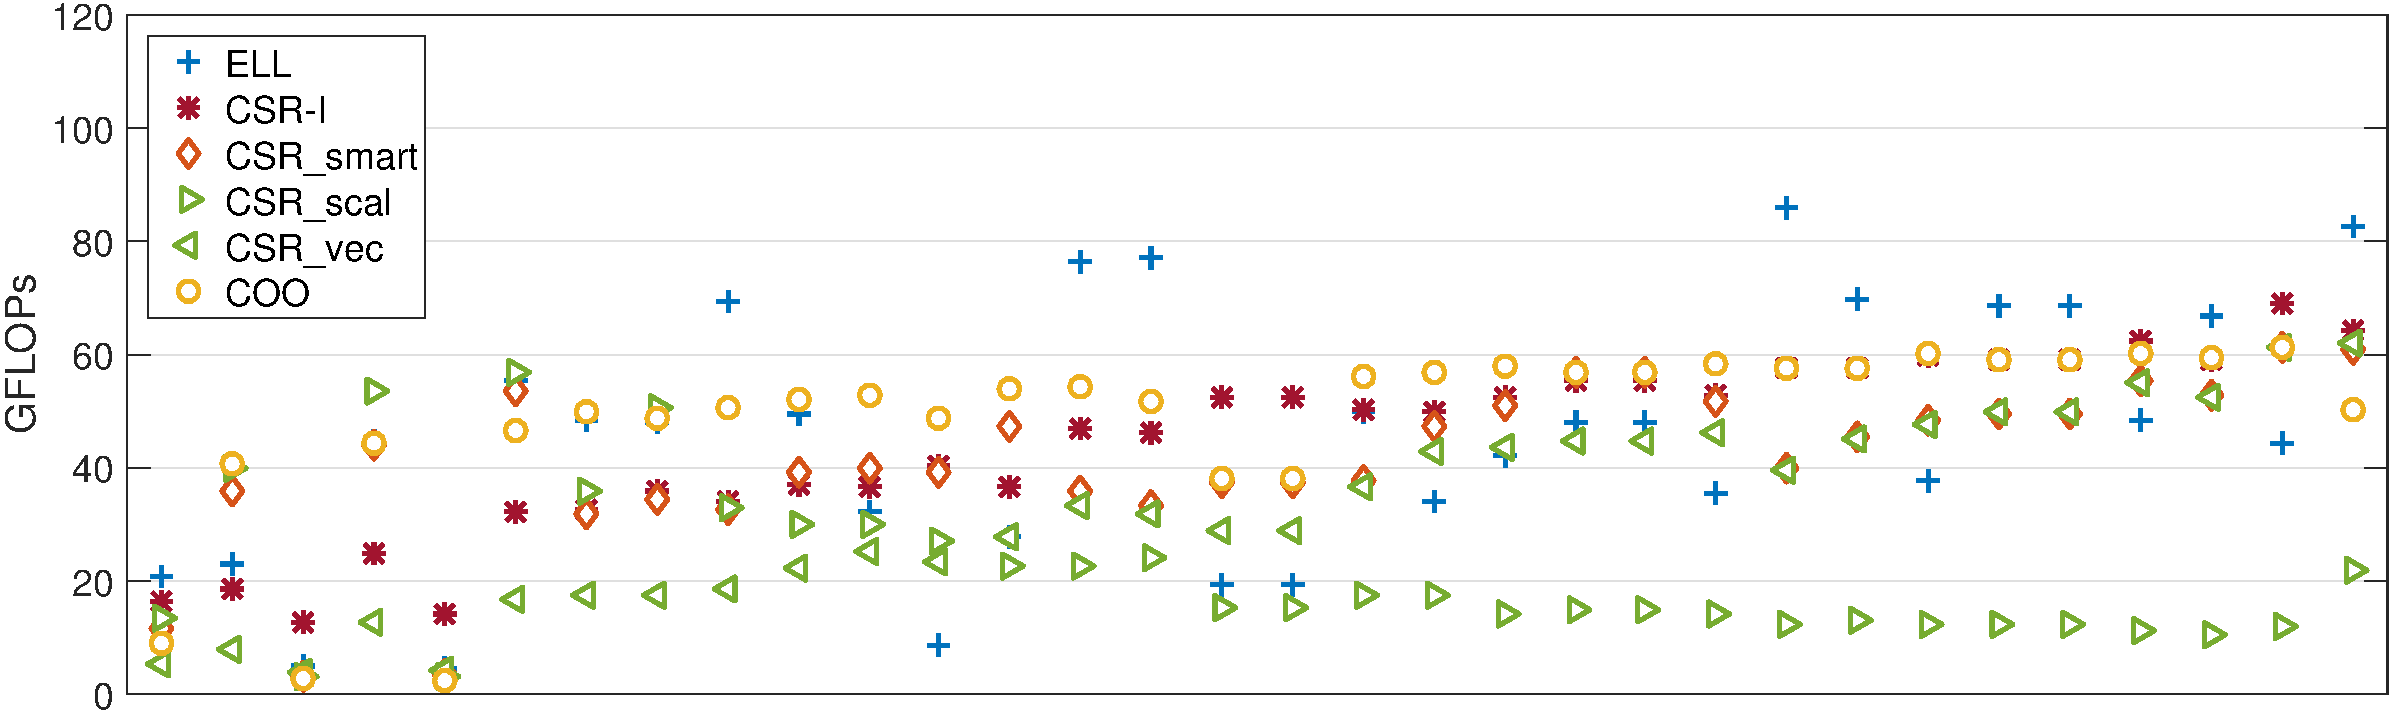
\includegraphics[width=0.9\columnwidth]{plots/SPARSE_GFLOPS}\\
			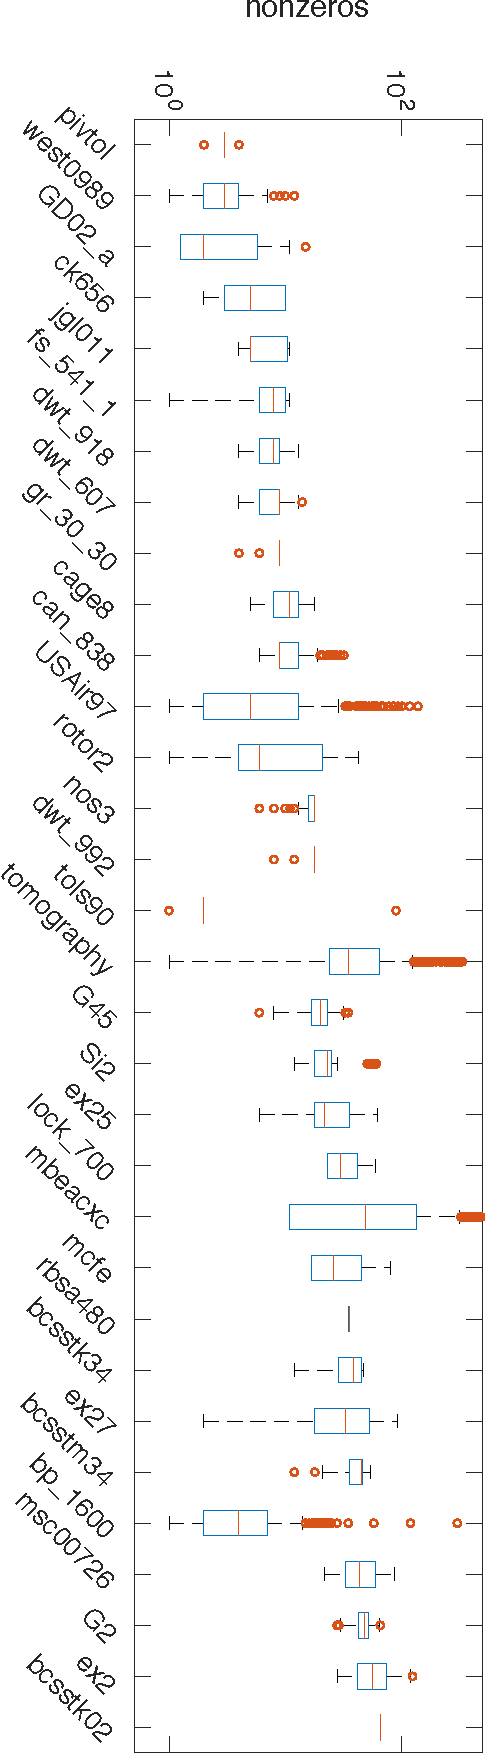
\includegraphics[width=.2527\columnwidth,angle=90]
                {plots/nnz_distribution_new}
		\end{tabular}
	\end{center}
	\caption
    [Performance of the flexible batched \spmv routines for all matrices in the
    test benchmark]
    {Performance of the flexible batched \spmv routines for all matrices in 
		the test 
		benchmark
		ordered in increasing nonzero-per-row ratio.
	}
	\label{2017-batched-spmv:fig:allmatricesperf}
\end{figure}


\subsection{Experimental results}
We first quantify the benefits of leveraging custom-designed batched kernels 
over the standard \spmv routines when processing batches of small matrices. 
For this purpose, we select 12 problems with between 800 and 1,024 unknowns 
from the test benchmark, and create
homogeneous batches.
In Figure~\ref{2017-batched-spmv:fig:selectperf} we visualize the performance achieved by
the standard \spmv routines versus the flexible batched \spmv kernels when
processing batches of increasing size.
In order to process a batch with multiple matrices via the standard \spmv 
kernels, we loop over the kernel invocations.
For the standard CSR kernel, MAGMA-sparse simply interfaces to NVIDIA's 
cuSPARSE library~\cite{cuda8.0};
the standard ELL kernel is the implementation available in 
MAGMA-sparse~\cite{sellpreport}.

The results of this experiment reveal
that the performance of the standard \spmv kernels never exceeds 5 GFLOPs.
Furthermore, although there is no clear winner among the batched \spmv kernels, 
they
all complete the operation at least 10$\times$ faster than their standard 
counterparts. 
For balanced problems, such as {\sc dwt992}, {\sc gr\_30\_30}, and {\sc nos3},
the performance of the \ell kernel surpasses 70 GFLOPs, a rate which is 
unmatched by any other kernel.
At the other end of the spectrum, the \csri kernel achieves very good 
performance for unbalanced
problems containing many nonzero elements, such as {\sc ex25} and {\sc msc}.
In these cases, the \ell kernel suffers from a significant zero-padding 
overhead.
For the very sparse problem {\sc west0989} the fastest options are \csrscal and 
\coo.
Overall, we acknowledge that the \coo kernel achieves very good performance 
across the complete test suite. In addition to being the fastest option in most 
of the cases, the \coo kernel
is the second-best choice in all remaining cases where a different format is 
superior.

\begin{figure}[t]
	\begin{center}
		\begin{tabular}{cc}
			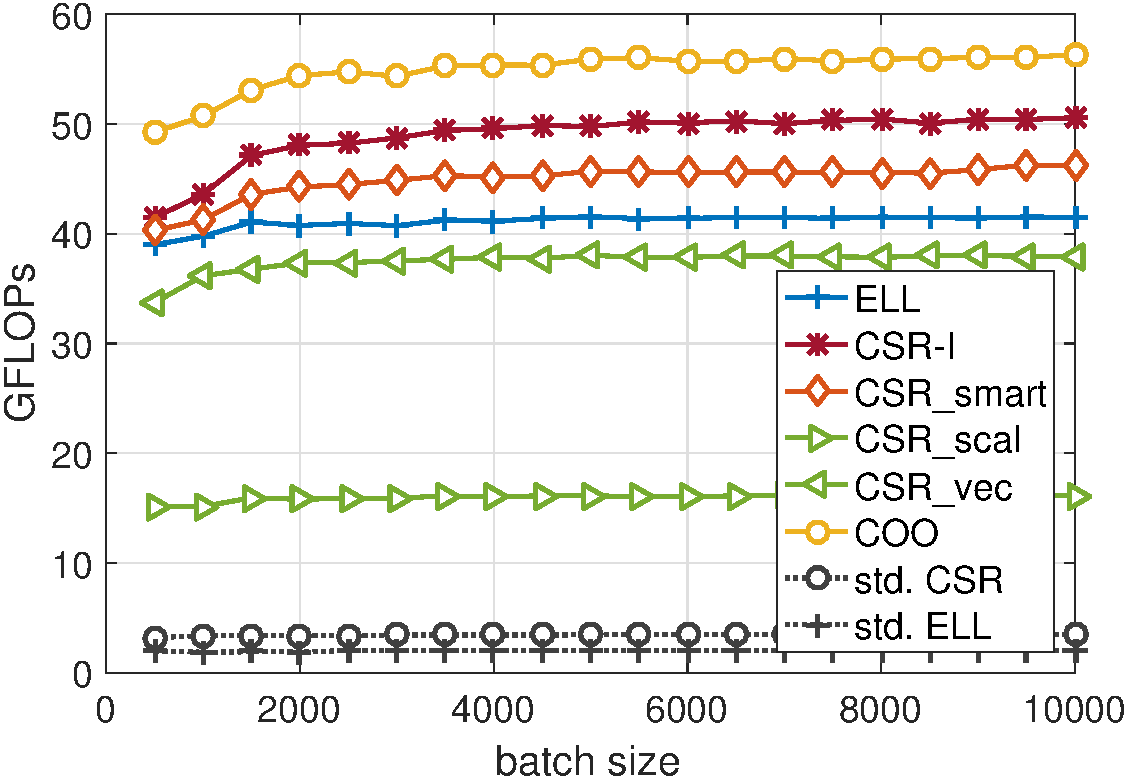
\includegraphics[width=.45\columnwidth]{plots/RND_UNITSIZE_GFLOPS}
			&
			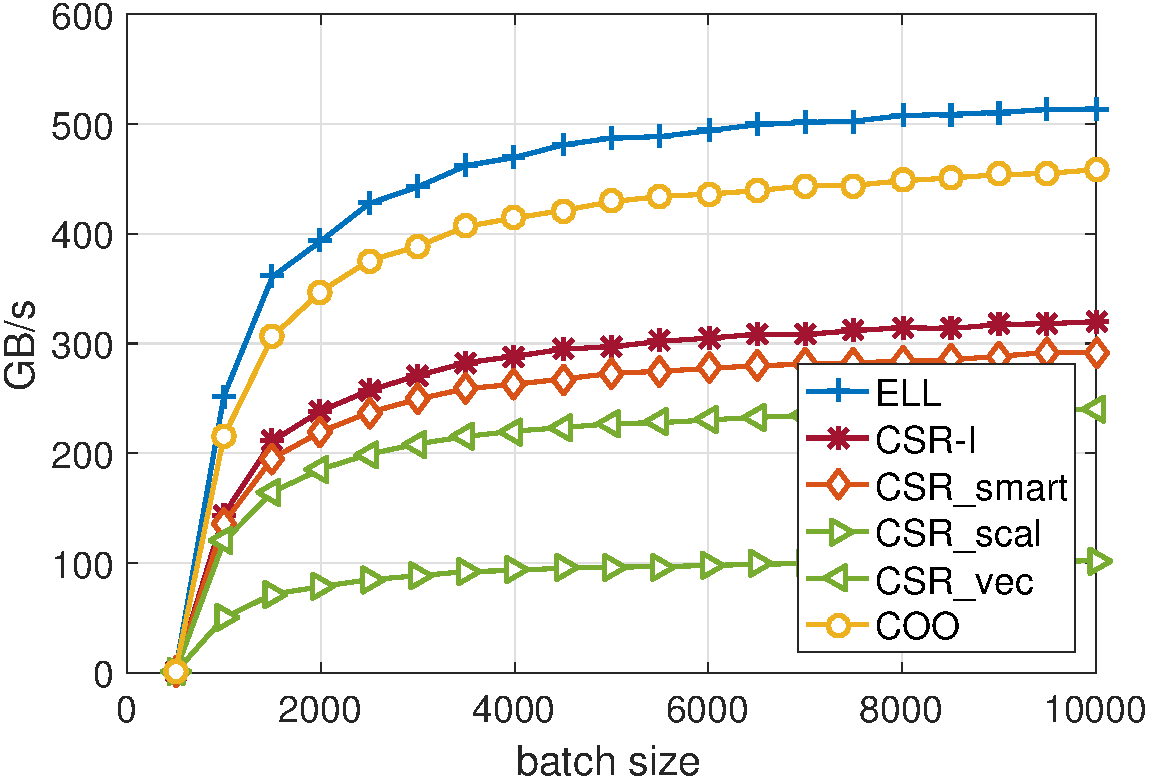
\includegraphics[width=.45\columnwidth]{plots/RND_UNITSIZE_BW}\\
		\end{tabular}
	\end{center}
	\caption
    [Performance and memory bandwidth of \spmv for a heterogeneous batch using
    selected matrices]
    {Performance (left) and sustained memory bandwidth (right) of the 
		flexible batched \spmv routines
		applied to a heterogeneous batch consisting of a random compilation of 
		the 
		matrices analyzed in Figure~\ref{2017-batched-spmv:fig:selectperf}.
	}
	\label{2017-batched-spmv:fig:similarsize}
\end{figure}

Next, we focus on the CSR format, for which we developed four kernels that 
differ in how they balance the workload.
For reference, we also include the standard CSR \spmv from NVIDIA's cuSPARSE in 
this analysis.
For the next experiment we generate a homogeneous batch containing 1,000 square 
matrices 
of size $1,024$
and vary the density and nonzero distribution.
We analyze the performance in relation to the average number of nonzero 
elements per row.
On the left-hand side of Figure~\ref{2017-batched-spmv:fig:incdensity}, we test a balanced 
nonzero distribution. 
The results show that the batched \csrscal offers very good performance for low 
nonzero-per-row ratios.
This comes from the fact that the data reads are mostly coalescent. The 
performance of \csrscal
drops in case there are more than 4 nonzeros per row, while the performance of 
\csrvec continues to improve.
\csrsmart  is a good trade-off between \csrscal and \csrvec, as it provides 
between 35 and 60 GFLOPs 
for most of the tested scenarios. 
The sequence of standard CSR \spmv calls never delivers more than 5 GFLOPs.
Especially for increasing nonzero count, the performance of \csri is 
competitive or even superior to \csrsmart.
However, for low nonzero-per-row ratios, \csrscal and \csrsmart are faster.
Conversely, on the right-hand side plot of Figure~\ref{2017-batched-spmv:fig:incdensity}, \csri 
gives the best performance
in all cases. This is expected as this experiment configures 
a batch of extremely unbalanced matrices with the nonzeros accumulated in a few 
rows. 
We recall that the good performance that \csri achieves for this problem comes 
at the price of a preprocessing
step to calculate the balancing information.

In Figure~\ref{2017-batched-spmv:fig:allmatricesperf} we analyze the performance of the flexible 
batched \spmv
kernels achieved for a homogeneous batch of 10000 matrices of the test 
benchmark.
The matrices are ordered in the $x$-axis 
according to increasing nonzero-per-row ratio. 
A larger value of this parameter 
makes the \csrscal kernel less attractive while the performance 
of \csrvec increases with the density. 
\csri and \csrsmart outperform \csrvec and \csrscal in most cases. 
None of the CSR-based kernels is competitive to the \coo kernel, which 
can be identified as overall winner in this experiment.
Only for balanced matrices, the \ell kernel outperforms all other competitors.
However, the performance of \ell is very problem-dependent, and for 
unbalanced nonzero distributions, it yields low performance.




\begin{figure}[t]
\begin{center}
\begin{tabular}{cc}
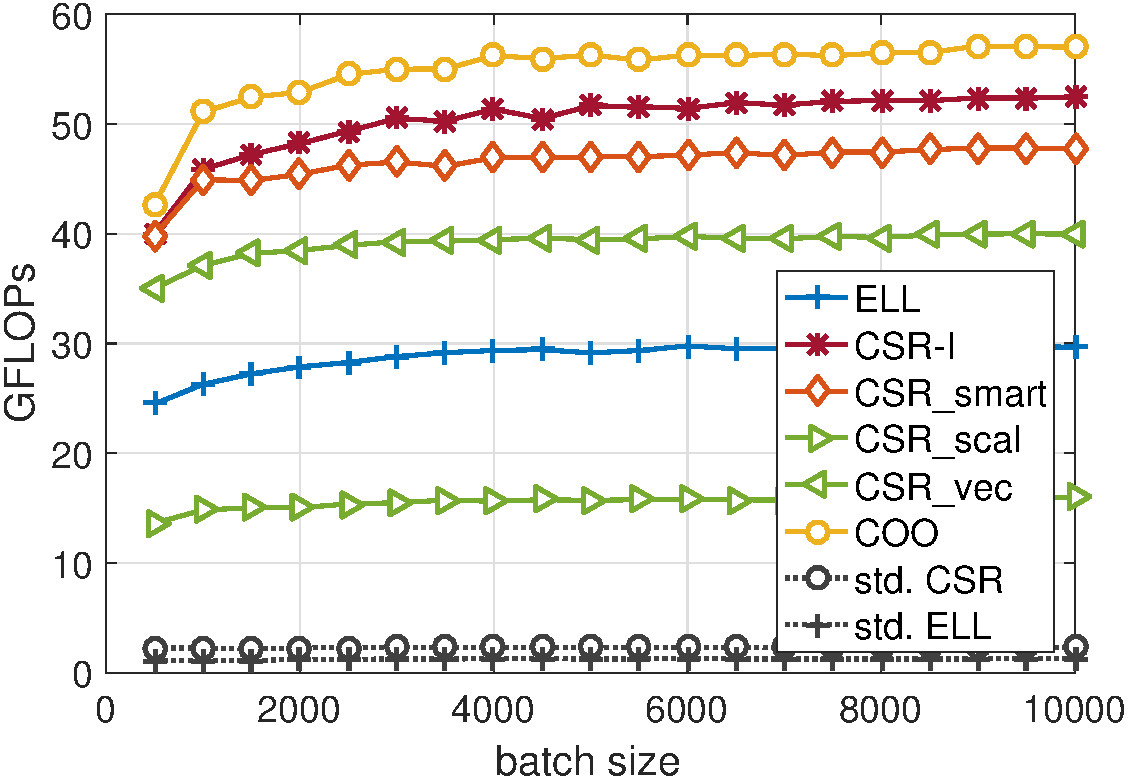
\includegraphics[width=.45\columnwidth]{plots/RND_GFLOPS}
&
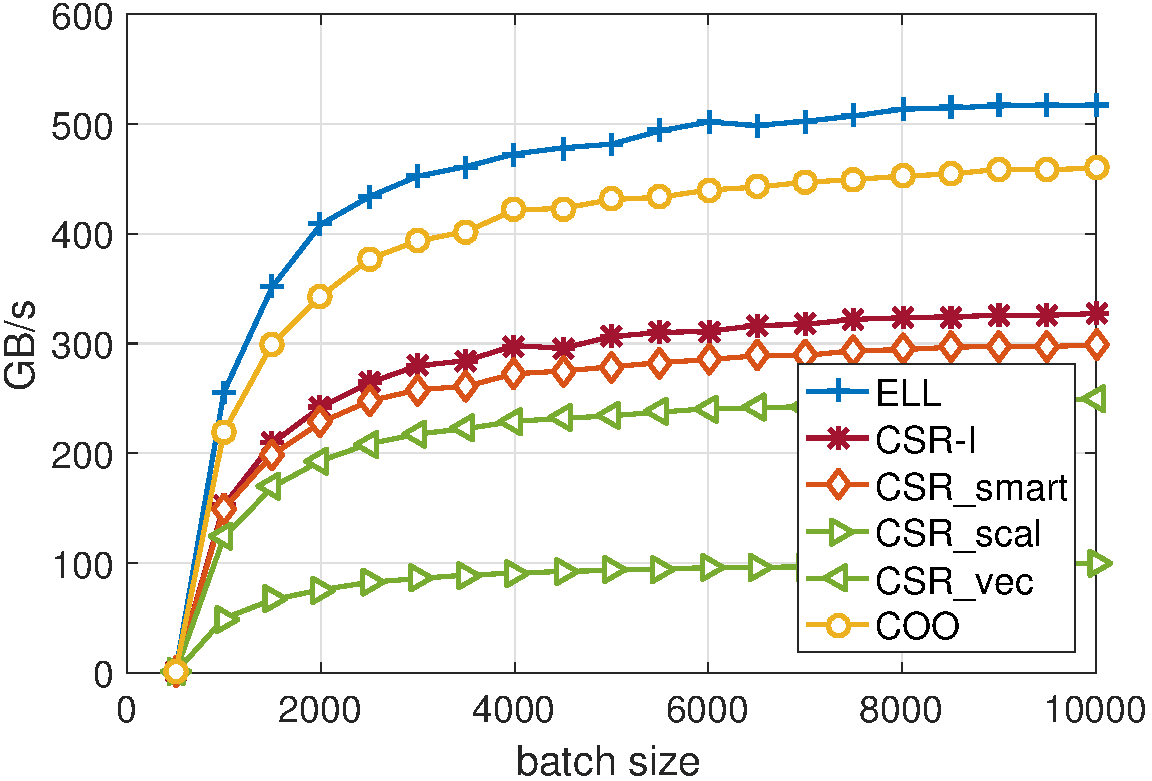
\includegraphics[width=.45\columnwidth]{plots/RND_BW}\\
\end{tabular}
\end{center}
\caption
[Performance and memory bandwidth of \spmv for a heterogeneous batch using all
matrices]
{Performance (left) and sustained memory bandwidth (right) of the 
flexible batched \spmv routines
applied to a heterogeneous batch consisting of a random compilation of all the 
matrices in the test benchmark.
}
\label{2017-batched-spmv:fig:allsize}
\end{figure}



We now turn to heterogeneous batches. First, we compose a batch with the 
matrices
we analyzed in Figure~\ref{2017-batched-spmv:fig:selectperf}. These matrices are very different 
in their nonzero pattern, 
but they all share similar size (800--1024 rows/columns).
In Figure~\ref{2017-batched-spmv:fig:similarsize} we show performance (left) and bandwidth 
(right) for the distinct 
batched \spmv kernels. In the latter, we also account for explicit zeros read 
into the multiprocessors.
We notice that the \ell kernel achieves memory access rates beyond 500 GB/s, 
which is about 70\% of the theoretical peak~\cite{P100}. 
\coo attains around 450 GB/s; and \csrsmart and \csri deliver around 300 GB/s.
However, the memory bandwidth is not the relevant factor in terms of 
runtime performance and, although the \ell kernel was the performance
winner for selected problems in Figure~\ref{2017-batched-spmv:fig:selectperf},
it only achieves about 40 GFLOPs in this experiment.
Higher throughput is achieved by \csrsmart (45 GFLOPs), \csri (50 GFLOPs),
and \coo (55 GFLOPs).
We mention that it is possible to improve the \ell kernel by 
using the sliced ELL format instead~\cite{sellpreport}.
There, the overhead introduced from zero-padding is reduced
by enforcing the same nonzero count only for those rows located in the same 
block.
However, we refrain from this optimization step as we expect the benefit to be 
moderate:
the height of the distinct row-blocks should at least match the warp size (32), 
which is relatively large compared to the small matrices we focus on.

Finally, we consider batches containing all of the matrices  in the test 
benchmark,
arranged in random order. Figure~\ref{2017-batched-spmv:fig:allsize} (right) shows that the \ell 
kernel sustains
a memory access rate around 500 GB/s. At the same time, the performance drops 
from 
40  to 30 GFLOPs, which is likely due to the large number of small and 
unbalanced 
test matrices in the batch.
Conversely, the performance of the other formats is not affected,
and \csrsmart, \csri and \coo
exceed 45, 50 and 55 GFLOPs, respectively.

We conclude that across all sparsity formats, the \coo kernel achieves the best 
performance
for heterogeneous batches. If the batch consists of balanced matrices only, 
the \ell kernel becomes the preferred choice, achieving up to 80 GFLOPs. In a 
one-touch-only
scenario where all matrices are stored in CSR format, the \csrsmart kernel is 
the best option.
If a preprocessing step is justified by a high number of kernel invocations, 
the \csri kernel
is much faster for batches consisting of unbalanced problems.
